\chapter{Część teoretyczna}
\section{Wprowadzenie do projektu}
% Genezą powstania serwisu internetowego jest fakt, że istnieje duża grupa osób z psami, które z różnych przyczyn nie mają czasu na regularne spacery ze swoim pupilem. Dodatkową funkcjonalnością oferowaną przez aplikację jest możliwość wyprowadzania potrzebujących psów na spacer jako opiekun. Jest to opcja przeznaczona dla osób, które lubią zajmować się zwierzętami i mają więcej wolnego czasu, niż opiekunowie.
Inspiracją do stworzenia serwisu internetowego, omawianego w niniejszej pracy dyplomowej, było najbliższe środowisko autora. Po wielu rozmowach zauważono, że w obecnych czasach można spotkać coraz więcej właścicieli psów, którzy przez różne, często losowe sytuacje, nie mogą sobie pozwolić na regularne spacery ze swoimi zwierzętami. Ponad to można wyróżnić pewną grupę osób, często z kręgu uczniowskiego, które mają zamiłowanie do zajmowania się zwierzętami oraz znacząco więcej wolnego czasu, który mogły by przeznaczyć na spacery z psami. Po przeanalizowaniu rynku zauważono, że w Polsce nie istnieje żadna specjalistyczna aplikacja, oferująca możliwość udostępniania oraz zapisywania się na spacery dla osób potrzebujących.

Głównym czynnikiem, który wpłyną na wybór oraz zastosowanie technologii internetowej, była chęć autora do zapoznania się z popularnym wśród wielu firm stosem technologicznym do tworzenia serwisów internetowych oraz dotarcie do większej ilości potencjalnych klientów.

\section{Proces projektowania i implementacji}
Proces tworzenia aplikacji obejmował kilka etapów:
\begin{itemize}[leftmargin=1cm]
    \item Opracowanie wymagań funkcjonalnych oraz niefunkcjonalnych;
    \item Opracowanie widoków aplikacji;
    \item Opracowanie warstwy biznesowej po stronie backendu;
    \item Opracowanie warstwy dostępowej po stronie frontendu;
\end{itemize}

Organizacja pracy nad projektem odgrywa kluczowe znaczenie na każdym etapie implementacyjnym. Każde stadium projektu było zarządzany przy pomocy aplikacji Trello. Jest to darmowa aplikacja, pozwalająca na skuteczne kierowanie projektem przez jedną lub wiele osób, współpracujących ze sobą. Organizacja pracy polegała na tworzeniu tablic do poszczególnych etapów. Tablice były tworzone na podstawie tych używanych w metodologii Kanban. Następnie na początku każdego etapu były planowane zadania do zrobienia i wpisywane do aplikacji. Miało to na celu większą organizację oraz kontrolę nad projektem. Wczesne zaznajomienie się ze zwinnymi metodykami zarządzania produkcją jest obecnie cenione na rynku pracy, ponieważ wiele firm z sektoru IT używa ich na codzień.
\section{Wymagania funkcjonalne oraz niefunkcjonalne}

W pierwszym etapie projektowania serwisu został stworzony spis wymagań funkcjonalnych oraz niefunkcjonalnych. Miało to na celu pogrupowanie zadań na odpowiednie podetapy. Pozwoliło skupić się na kluczowych, dla danej fazy, funkcjach.
\subsection{Wymagania funkcjonalne}
\begin{itemize}
    \item Rejestracja nowych użytkowników z podziałem na role;
    \item Logowanie użytkowników do serwisu;
    \item Możliwość zmiany danych użytkownika -- zdjęcie profilowe, dane osobowe, hasło;
    \item Możliwość dodania profilu swojego psa;
    \item Możliwość stworzenia spaceru;
    \item Ocena opiekunów po zakończonym spacerze;
    \item Przeglądanie listy dostępnych spacerów;
    \item Przeglądanie listy nadchodzących spacerów;
    \item Zapisywanie na spacery;
    \item Wypisywanie się ze spacerów;
    \item Dodawanie opinii o wyprowadzonym zwierzaków;
    \item Przeglądanie historii spacerów;
    \item Przeglądanie profili uzytkowników;
    \item Przeglądanie profili spacerów;
    \item Zgłaszanie błędów w aplikacji przez użytkowników;
    \item Zarządzanie kontami użytkowników -- blokowanie, banowanie;
    \item Wyświetlanie bazy danych użytkowników;
    \item Wyświetlanie bazy danych zwierzaków;
    \item Wyświetlanie bazy danych spacerów;
    \item System zarządzania zgłoszonymi błędami;
\end{itemize}
\subsection{Wymagania niefunkcjonalne}
\begin{itemize}
    \item Dostęp do internetu;
\end{itemize}
\newpage
\section{Diagram oraz przypadki użycia}
\subsection{Diagramy użycia}
\begin{figure}[h]
    \centering
    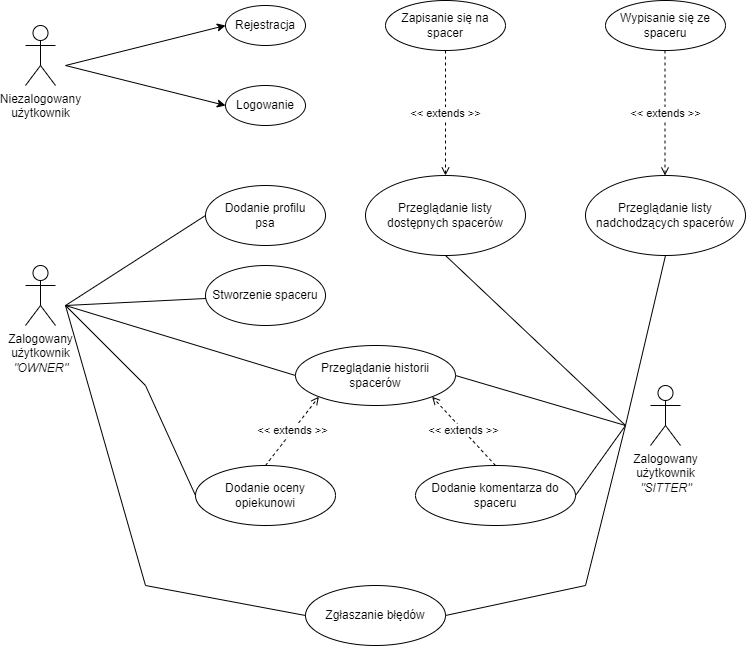
\includegraphics[width=0.7\linewidth]{rysunki/use-case.png}
    \caption{Diagram przypadków użycia}
    \label{fig:use-case-diagram}
\end{figure}    

\subsection{Przypadki użycia}
\noindent
\textbf{Przypadek użycia:} Rejestracja. \\
\textbf{Aktor:} Niezalogowany użytkownik. \\
\textbf{Opis:} Rejestracja w serwisie. \\
\textbf{Warunki wstępne:} Użytkownik niezalogowany, nieposiadający konta, wchodzący do serwisu po raz pierwszy.\\
\textbf{Przebieg:}
\begin{itemize}[leftmargin=1cm]
    \item Użytkownik klika w odnośnik \textit{...};
    \item Użytkownik zostaje przeniesiony do strony z formularzem rejestracyjnym;
    \item  Użytkownik wypełnia dane;
    \begin{itemize}
        \item Dane są niepoprawne -- serwis informuje uzytkownika o błędach, przycisk jest nieaktywny;
        \item Dane są poprawne -- przycisk jest aktywny i użytkownik może stworzyć konto;
    \end{itemize}
    \item Wysłanie formularzu -- użytkownik jest informowany o sukcesie bądź błędzie operacji;
\end{itemize}

\textbf{Przypadek użycia:} Logowanie. \\
\textbf{Aktor:} Niezalogowany użytkownik. \\
\textbf{Opis:} Logowanie do serwisu. \\
\textbf{Warunki wstępne:} Użytkownik niezalogowany, posiadający konto w serwisie. \\
\textbf{Przebieg:}
\begin{itemize}[leftmargin=1cm]
    \item Użytkownik wypełnia formularz logowania;
    \item Użytkownik klika w przycisk \textit{Zaloguj się};
    \begin{itemize}
        \item W przypadku sukcesu użytkownik zostaje przekierowany do strony aplikacji;
        \item W przypadku błędu użytkownik jest informowany o błędzie;
    \end{itemize}
\end{itemize}

\noindent
\textbf{Przypadek użycia:} Zmiana zdjęcia profilowego. \\
\textbf{Aktor:} Zalogowany użytkownik. \\
\textbf{Opis:} Zmiana zdjęcia profilowego. \\
\textbf{Warunki wstępne:} Użytkownik zalogowany z aktywnym kontem. \\
\textbf{Przebieg:}
\begin{itemize}[leftmargin=1cm]
    \item Użytkownik wchodzi w zakładkę profil;
    \item Po najechaniu na zdjęcie profilowe klika w ikonę edycji;
    \item Użytkownik wgrywa nowe zdjęcie;
    \item Użytkownik klika w przycisk \textit{Zmień zdjęcie};
    \item Użytkownik otrzymuje informację zwrotną o statusie wykonanej operacji;
\end{itemize}

% \textbf{Przypadek użycia:} Zmiana opisu. \\
% \textbf{Aktor:} Zalogowany użytkownik. \\
% \textbf{Opis:} Zmiana opisu profilu. \\
% \textbf{Warunki wstępne:} Użytkownik zalogowany z aktywnym kontem. \\
% \textbf{Przebieg:}
% \begin{itemize}
%     \item Użytkownik wchodzi w zakładkę profil
%     \item Po najechaniu na opis profilowe klika w ikonę edycji
%     \item Użytkownik wypełnia formularz
%     \item Użytkownik klika w przycisk "Zmień opis"
%     \item Użytkownik otrzymuje informację zwrotną o statusie wykonanej operacji
% \end{itemize}

% \textbf{Przypadek użycia:} Zmiana danych. \\
% \textbf{Aktor:} Zalogowany użytkownik. \\
% \textbf{Opis:} Zmiana danych. \\
% \textbf{Warunki wstępne:} Użytkownik zalogowany z aktywnym kontem. \\
% \textbf{Przebieg:}
% \begin{itemize}
%     \item Użytkownik wchodzi w zakładkę profil
%     \item Po najechaniu na dane klika w ikonę edycji
%     \item Użytkownik wypełnia formularz
%     \item Użytkownik klika w przycisk "Zmień dane"
%     \item Użytkownik otrzymuje informację zwrotną o statusie wykonanej operacji
% \end{itemize}

% \textbf{Przypadek użycia:} Zmiana hasła. \\
% \textbf{Aktor:} Zalogowany użytkownik. \\
% \textbf{Opis:} Zmiana hasła. \\
% \textbf{Warunki wstępne:} Użytkownik zalogowany z aktywnym kontem. \\
% \textbf{Przebieg:}
% \begin{itemize}
%     \item Użytkownik wchodzi w zakładkę profil
%     \item Po najechaniu na dane klika w ikonę edycji
%     \item Użytkownik wypełnia formularz
%     \item Użytkownik klika w przycisk "Zmień hasło"
%     \item Użytkownik otrzymuje informację zwrotną o statusie wykonanej operacji
% \end{itemize}

\noindent
\textbf{Przypadek użycia:} Dodanie profilu psa. \\
\textbf{Aktor:} Zalogowany użytkownik. \\
\textbf{Opis:} Dodanie profilu zwierzaka do serwisu. \\
\textbf{Warunki wstępne:} Użytkownik zalogowany, z aktywnym kontem oraz rolą \textit{OWNER}. \\
\textbf{Przebieg:}
\begin{itemize}[leftmargin=1cm]
    \item Użytkownik wchodzi w zakładkę \textit{Dodaj spacer};
    \item Użytkownik wypełnia formularz;
    \begin{itemize}
        \item Dane są poprawne -- aktywuje się submit button (przypis);
        \item Dane są niepoprawne -- pojawia się informacja zwrotna;
    \end{itemize}
    \item Użytkownik klika w przycisk \textit{Dodaj zwierzaka};
    \begin{itemize}
        \item W przypadku sukcesu użytkownik zostaje przekierowany do strony aplikacji;
        \item W przypadku błędu użytkownik jest informowany o błędzie;
    \end{itemize}
\end{itemize}

\noindent
\textbf{Przypadek użycia:} Dodanie nowego spaceru. \\
\textbf{Aktor:} Zalogowany użytkownik. \\
\textbf{Opis:} Dodanie terminu spaceru. \\
\textbf{Warunki wstępne:} Użytkownik zalogowany, z aktywnym kontem oraz rolą \textit{OWNER}. \\
\textbf{Przebieg:}
\begin{itemize}[leftmargin=1cm]
    \item Użytkownik wchodzi w zakładkę \textit{Dodaj spacer};
    \item Użytkownik wypełnia formularz;
    \begin{itemize}
        \item Dane są poprawne -- aktywuje się submit button (przypis);
        \item Dane są niepoprawne -- pojawia się informacja zwrotna;
    \end{itemize}
    \item Użytkownik klika w przycisk \textit{Dodaj zwierzaka};
    \begin{itemize}
        \item W przypadku sukcesu użytkownik zostaje przekierowany do strony aplikacji;
        \item W przypadku błędu użytkownik jest informowany o błędzie;
    \end{itemize}
\end{itemize}

\noindent
\textbf{Przypadek użycia:} Przeglądanie historii spacerów. \\
\textbf{Aktor:} Zalogowany użytkownik. \\
\textbf{Opis:} Przeglądanie historii spacerów. \\
\textbf{Warunki wstępne:} Zalogowany użytkownik z aktywnym kontem oraz rolą \textit{OWNER} lub \textit{SITTER}. \\
\textbf{Przebieg:}
\begin{itemize}[leftmargin=1cm]
    \item Użytkownik wchodzi w zakładkę \textit{Historia};
    \item Wyświetlana jest lista spacerów w przszłości;
\end{itemize}

\noindent
\textbf{Przypadek użycia:}  Skomentowanie spaceru. \\
\textbf{Aktor:} Zalogowany użytkownik. \\
\textbf{Opis:} Dodanie komentarza do spaceru. \\
\textbf{Warunki wstępne:} Zalogowany użytkownik z aktywnym kontem, rolą \textit{SITTER} oraz spacerem w przeszłości. \\
\textbf{Przebieg:}
\begin{itemize}[leftmargin=1cm]
    \item Uzytkownik wchodzi w zakładkę \textit{Historia};
    \item Użytkownik wybiera spacer, który chce skomentować;
    \item Użytkownik wypełnia formularz;
    \begin{itemize}
        \item Dane są poprawne -- aktywuje się submit button (przypis);
        \item Dane są niepoprawne -- pojawia się informacja zwrotna;
    \end{itemize}
    \item Użytkownik klika w przycisk \textit{Dodaj komentarz};
    \begin{itemize}
        \item W przypadku sukcesu użytkownik zostaje przekierowany do strony aplikacji;
        \item W przypadku błędu użytkownik jest informowany o błędzie;
    \end{itemize}
\end{itemize}

\noindent
\textbf{Przypadek użycia:} Ocena opiekuna. \\
\textbf{Aktor:} Zalogowany użytkownik. \\
\textbf{Opis:} Dodanie oceny opiekunowi. \\
\textbf{Warunki wstępne:}  Zalogowany użytkownik z aktywnym kontem, rolą \textit{OWNER} oraz zakończonym spacerem w przeszłości. \\
\textbf{Przebieg:}
\begin{itemize}[leftmargin=1cm]
    \item Uzytkownik wchodzi w zakładkę \textit{Historia};
    \item Użytkownik wybiera spacer z opiekunem, którego chce ocenić;
    \item Użytkownik wypełnia formularz;
    \begin{itemize}
        \item Dane są poprawne -- aktywuje się submit button (przypis);
        \item Dane są niepoprawne -- pojawia się informacja zwrotna;
    \end{itemize}
    \item Użytkownik klika w przycisk \textit{Dodaj ocenę};
    \begin{itemize}
        \item W przypadku sukcesu użytkownik zostaje przekierowany do strony aplikacji;
        \item W przypadku błędu użytkownik jest informowany o błędzie;
    \end{itemize}
\end{itemize}

\noindent
\textbf{Przypadek użycia:} Przeglądanie listy dostępnych spacerów. \\
\textbf{Aktor:} Zalogowany użytkownik. \\
\textbf{Opis:}  Przeglądanie listy dostępnych spacerów. \\
\textbf{Warunki wstępne:} Zalogowany użytkownik z aktywnym kontem oraz rolą \textit{SITTER}. \\
\textbf{Przebieg:}
\begin{itemize}[leftmargin=1cm]
    \item Użytkownik wchodzi w zakładkę \textit{Spacery} z aktywnym widokiem wszystkich spacerów;
    \item Pobierana jest lista psów, bazująca na lokalizacji;
    \item Lista spacerów wyświetlana jest użytkownikowi;
\end{itemize}

\noindent
\textbf{Przypadek użycia:} Zapisanie się na spacer. \\
\textbf{Aktor:} Zalogowany użytkownik. \\
\textbf{Opis:} Zapisanie się na spacer. \\
\textbf{Warunki wstępne:} Zalogowany uzytkownik z aktywnym kontem, rolą \textit{SITTER} oraz spacer dostępny w przyszłości z wolnym miejscem do zapisu. \\
\textbf{Przebieg:}
\textbf{Scenariusz A: Użytkownik znajduje się w zakładce \textit{Spacery}}
\begin{itemize}[leftmargin=1cm]
    \item Użytkownik klika w przycisk \textit{Zapisz się};
    \item Użytkownik jest informowany stosownym komunikatem;
\end{itemize}
\textbf{Scenariusz B: Użytkownik znajduje się w profilu spaceru}
\begin{itemize}[leftmargin=1cm]
    \item Użytkownik klika w przycisk \textit{Zapisz się};
    \item Użytkownik jest informowany stosownym komunikatem;
\end{itemize}

\noindent
\textbf{Przypadek użycia:} Wypisanie się ze spaceru. \\
\textbf{Aktor:} Zalogowany użytkownik. \\
\textbf{Opis:} Wypisanie się ze spaceru. \\
\textbf{Warunki wstępne:} Zalogowany uzytkownik z aktywnym kontem, rolą \textit{SITTER} oraz spacer w przyszłości na który użytkownik jest już zapisany. \\
\textbf{Przebieg:}
\textbf{Scenariusz A: Użytkownik znajduje się w zakładce \textit{Spacery}}
\begin{itemize}[leftmargin=1cm]
    \item Użytkownik klika w przycisk \textit{Wypisz się};
    \item Użytkownik jest informowany stosownym komunikatem;
\end{itemize}
\textbf{Scenariusz B: Użytkownik znajduje się w profilu spaceru}
\begin{itemize}[leftmargin=1cm]
    \item Użytkownik klika w przycisk \textit{Wypisz się};
    \item Użytkownik jest informowany stosownym komunikatem;
\end{itemize}

\noindent
\textbf{Przypadek użycia:} Przeglądanie listy nadchodzących spacerów. \\
\textbf{Aktor:} Zalogowany uzytkownik. \\
\textbf{Opis:} Przeglądanie listy nadchodzących spacerów na które użytkownik jest zapisany. \\
\textbf{Warunki wstępne:} Zalogowany uzytkownik z aktywnym kontem, rolą \textit{SITTER} oraz co najmniej jednym spacerem na który jest zapisany. \\
\textbf{Przebieg:}
\begin{itemize}[leftmargin=1cm]
    \item Uzytkownik wchodzi w zakładkę \textit{Spacery};
    \item Uzytkownik przełącza widok na \textit{Nadchodzące};
    \item Lista nadchodzących spacerów jest wyświetlana użytkownikowi;
\end{itemize}

\noindent
\textbf{Przypadek użycia:} Przeglądanie terminarza ze spacerami. \\
\textbf{Aktor:} Zalogowany użytkownik. \\
\textbf{Opis:} Przeglądanie terminarza ze spacerami, na które użytkownik jest zapisany. \\
\textbf{Warunki wstępne:} Zalogowany użytkownik z aktywnym kontem oraz rolą \textit{SITTER}. \\
\textbf{Przebieg:}
\begin{itemize}[leftmargin=1cm]
    \item Użytkownik wchodzi w zakładkę \textit{Terminarz};
    \item Uzytkownik może wybrać tryb wyświetlania;
    \begin{itemize}
        \item Miesiąc -- widok miesiąca ze zdjęciami psów oraz odnośnikami do profilu spaceru;
        \item Tydzień -- widok tygodniowy z podstawowymi informacjami o danym spacerze oraz odnośnikiem do profilu spaceru;
    \end{itemize}
\end{itemize}

\noindent
\textbf{Przypadek użycia:} Przeglądanie profilu uzytkownika. \\
\textbf{Aktor:} Zalogowany użytkownik. \\
\textbf{Opis:} Przeglądanie profilu użytkownka. \\
\textbf{Warunki wstępne:} Zalogowany użytkownik z aktywnym kontem oraz dowolną rolą. \\
\textbf{Przebieg:}
\begin{itemize}[leftmargin=1cm]
    \item Użytkownik klika w odnośnik przekierowujący na profil innego użytkownika;
    \item Wyświetlają się szczegółowe informacje o użytkowniku;
\end{itemize}

\noindent
\textbf{Przypadek użycia:} Przeglądanie profilu psa. \\
\textbf{Aktor:} Zalogowany użytkownik. \\
\textbf{Opis:} Przeglądanie profilu psa. \\
\textbf{Warunki wstępne:} Zalogowany użytkownik z aktywnym kontem oraz dowolną rolą. \\
\textbf{Przebieg:}
\begin{itemize}[leftmargin=1cm]
    \item Uzytkownik klika w odnośnik przekierowujący na profil psa;
    \item Wyświetlają się szczegółowe informacje;
\end{itemize}

\noindent
\textbf{Przypadek użycia:} Przeglądanie profilu spaceru. \\
\textbf{Aktor:} Zalogowany użytkownik. \\
\textbf{Opis:} Przeglądanie profilu spaceru. \\
\textbf{Warunki wstępne:} Zalogowany użytkownik z aktywnym kontem oraz dowolną rolą. \\
\textbf{Przebieg:}
\begin{itemize}[leftmargin=1cm]
    \item Użytkownik klika w odnośnik przekierowujący na profil spaceru;
    \item Wyświetlają się szczegółowe informacje o spacerze;
\end{itemize}

\noindent
\textbf{Przypadek użycia:} Zgłaszanie błędów. \\
\textbf{Aktor:} Zalogowany użytkownik. \\
\textbf{Opis:}  Zalogowany użytkownik. \\
\textbf{Warunki wstępne:} Zalogowany użytkownik z aktywnym kontem oraz dowolną rolą. \\
\textbf{Przebieg:}
\begin{itemize}[leftmargin=1cm]
    \item Użytkownik klika w ikonę błędu w prawym dolnym rogu;
    \item Użytkownik wypełnia formularz;
    \begin{itemize}
        \item Dane są poprawne -- aktywuje się submit button (przypis);
        \item Dane są niepoprawne -- pojawia się informacja zwrotna;
    \end{itemize}
    \item Użytkownik klika w przycisk \textit{Zgłoś błąd};
    \begin{itemize}
        \item W przypadku sukcesu użytkownik zostaje przekierowany do strony aplikacji;
        \item W przypadku błędu użytkownik jest informowany o błędzie;
    \end{itemize}
\end{itemize}

\noindent
\textbf{Przypadek użycia:} Przeglądanie listy wszystkich użytkowników. \\
\textbf{Aktor:} Zalogowany użytkownik. \\
\textbf{Opis:} Przeglądanie bazy użytkowników. \\
\textbf{Warunki wstępne:} Zalogowany użytkownik z rolą \textit{ADMIN}. \\
\textbf{Przebieg:}
\begin{itemize}[leftmargin=1cm]
    \item Użytkownik wchodzi w zakładkę \textit{Użytkownicy};
    \item Pojawia się lista wszystkich użytkowników zarejestrowanych w serwisie;
\end{itemize}

\noindent
\textbf{Przypadek użycia:} Przeglądanie listy wszystkich spacerów. \\
\textbf{Aktor:} Zalogowany użytkownik. \\
\textbf{Opis:} Przeglądanie bazy spacerów. \\
\textbf{Warunki wstępne:} Zalogowany użytkownik z rolą \textit{ADMIN}. \\
\textbf{Przebieg:}
\begin{itemize}[leftmargin=1cm]
    \item Użytkownik wchodzi w zakładkę \textit{Zwierzęta i spacery};
    \item Użytkownik wybiera widok spacerów;
    \item Pojawia się lista wszystkich spacerów dodanych w serwisie;
\end{itemize}

\noindent
\textbf{Przypadek użycia:} Przeglądanie listy wszystkich psów . \\
\textbf{Aktor:} Zalogowany użytkownik. \\
\textbf{Opis:} Przeglądanie bazy zwierząt. \\
\textbf{Warunki wstępne:} Zalogowany użytkownik z rolą \textit{ADMIN}. \\
\textbf{Przebieg:}
\begin{itemize}[leftmargin=1cm]
    \item Użytkownik wchodzi w zakładkę \textit{Zwierzęta i spacery};
    \item Użytkownik wybiera widok zwierząt;
    \item Pojawia się lista wszystkich psów dodanych w serwisie;
\end{itemize}

\noindent
\textbf{Przypadek użycia:} Przeglądanie aktywności użytkowników. \\
\textbf{Aktor:} Zalogowany użytkownik. \\
\textbf{Opis:} Przeglądanie aktywności użytkowników. \\
\textbf{Warunki wstępne:} Zalogowany użytkownik z rolą \textit{ADMIN} . \\
\textbf{Przebieg:}
\begin{itemize}[leftmargin=1cm]
    \item Uzytkownik wchodzi w zakładkę \textit{Aktywność};
    \item Pojawia się lista aktywności użytkowników na serwisie;
\end{itemize}

\noindent
\textbf{Przypadek użycia:} Przeglądanie listy zgłoszonych błędów. \\
\textbf{Aktor:} Zalogowany użytkownik. \\
\textbf{Opis:} Przeglądanie listy zgłoszonych błędów przez użytkowników. \\
\textbf{Warunki wstępne:} Zalogowany użytkownik z rolą \textit{ADMIN}. \\
\textbf{Przebieg:}
\begin{itemize}[leftmargin=1cm]
    \item Użytkownik wchodzi w zakładkę \textit{Błędy};
    \item Pojawiają się lista błędów podzielona na 3 grupy -- nowe, w trakcie realizacji, naprawione;
\end{itemize}

\noindent
\textbf{Przypadek użycia:} Przeglądanie dashboardu (przypis). \\
\textbf{Aktor:} Zalogowany użytkownik. \\
\textbf{Opis:} Przeglądanie dashboardu. \\
\textbf{Warunki wstępne:} Zalogowany uzytkownik z rolą \textit{OWNER} lub \textit{SITTER}. \\
\textbf{Przebieg:}
\begin{itemize}[leftmargin=1cm]
    \item Użytkownik znajduje się w zakładce dashboard;
    \item Pojawia się lista nadchodzących spacerów oraz powiadomień;
\end{itemize}

\section{Widoki, mockupy}
Kluczowym elementem przy projektowaniu serwisów internetowych jest stworzenie prototypu aplikacji. Prototypowanie przyszłej aplikacji pozwala w krótszym czasie zaprojektować atrakcyjny wygląd, zgodny z technikami UI/UX (\textit{ang. User Interface / User Expirience}).

W trakcie etapu projektowania zdecydowano się na użycie \textit{Adobe XD}. Jest to popularne narzędzie do prototypowania -- głównie na platformy internetowe oraz mobilne. Program pozwala na projektowanie makiet aplikacji poprzez wykorzystanie podstawowych kształtów oraz ich właściwości. Zaletą specjalistycznych narzędzi do prototypowania jest zastosowanie zbioru właściwości, które służą do nadawania poszczególnym elementom pożądanego wyglądu, znznych z często używanego narzędzia do stylizacji plików HTML -- kaskadowych arkuszy stylów. Takie rozwiązanie pozwala w błyskawiczny sposób przenieść prototypy do docelowego projektu.

% Ten zabieg znacząco ułatwia i przyspiesza pracę w etapie implementowania warstwy dostępowej. 

% Do stworzenia prototypów użyto oprogramowania \textit{Adobe XD}. Jest to popularne narzędzie do tworzenia interfejsów użytkownika. Program oferuje szereg narzędzi do projektowania wyglądu aplikacji. Zaletą używania programów, których przeznaczeniem jest kreowanie makiet aplikacji internetowych, jest zastosowanie właściwości dodawanych elementów znanych z arkuszy stylów takich, jak \textit{CSS} bądź \textit{SCSS}. Pozwala to w późniejszym czasie bezproblemowo przenosić zaprojektowane wyglądy do aplikacji frontendowej.
\section{Backend}
Każda aplikacja internetowa posiada swój silnik, który jest określany jako \textit{backend}. Jest to logika biznesowa, stojąca po stronie serwera. Odpowiada za pobieranie oraz przetwarzanie danych, komunikację z bazą danych oraz w większym stopniu za bezpieczeństwo całej aplikacji. Aplikacje backendowe udostępniają zbiór funkcjonalności, inaczej zwane REST API \textit{(ang. ...)}, które są wykorzystywane do transferu danych między zapleczem technicznym a warstwą dostępową aplikacji internetowej.

W omawianej aplikacji do implementacji backendu wykorzystano język \textit{Java} - popularny język obiektowy oparty na klasach, charakteryzujący się kodem, który po kompilacji można uruchomić na każdej platformie. Niezbędny był również framework \textit{Spring Boot}, dzięki któremu możliwe było stworzenie rozbudowanego API aplikacji. Spring Boot jest narzędziem opartym o framework \textit{Spring}, zapewniającym dodatkową konfigurację oraz kontener aplikacji. Takie zastosowanie pozwala na szybsze tworzenie aplikacji bez konieczności dodatkowej konfiguracji. Użyty framework korzysta z mechanizmu wstrzykiwania zależności \textit{(ang. Dependency Injection)}. Dependency injection odpowiada za tworzenie i dostarczanie obiektów w odpowiednim momencie do danej klasy. Obecnie Java w połączeniu ze Spring Boot'em jest powszechnie używanym narzędziem wśród wielu firm na całym świecie. 

Do tworzenia warstw biznesowych przy wykorzystaniu wyżej wymienionch narzędzi, niezbędnym elementem jest zbiór zależności. Pozwalają rozszerzyć bazowe funkcjonalności o nowe, skonkretyzowane metody i rozwiązania. W przypadku aplikacji, która jest tematem niniejszej pracy wykorzystano nastepujące zależności:
\begin{itemize}[leftmargin=1cm]
    \item \textbf{Spring Web} -- wprowadza do projektu podstawowe funkcje integracyjne, inicjalizuje kontener IoC, zorientowuje kontekst aplikacji na sieć oraz dodaje klienta HTTP.
    \item \textbf{Spring Security} -- konfigurowalna platforma zapewniająca kontrolę nad dostępem do aplikacji. Stanowi standard zabezpieczeń oraz pozwala na uwierystelnianie użytkowników.
    \item \textbf{JSON Web Token} -- popularne rozwiązanie do uwierzytelniania użytkowników. Wykorzystywany jako token autoryzacyjny, generowany po stronie backendu i przechowywany po stronie frontendu, umożliwia na dostęp do zasobów API aplikacji.
    \item \textbf{MongoDB Driver} -- zależność umożliwiająca skonfigurowanie aplikacji z bazą danych. Udostępnia szereg metod umożliwiający wykonywanie operacji z przetwarzaniem danych w bazie.
    \item \textbf{SwaggerUI} -- dostarcza wizualną reprezentację oraz dostęp do punktów końcowych \textit{(ang. endpoint)} aplikacji. Umożliwia na testowanie zaimplementowanych funkcjonalności bezpośrednio po stronie backendu.
    \item \textbf{Lombok} -- jest procesorem adnotacji, umożiwiającym na generowanie kodu przed kompilacją po zastosowaniu odpowiedniej adnotacji nad klasą. Wykorzystywany jest przy obiektach do generowania powtarzalnych metod takich jak konstuktory, gettery oraz settery.
\end{itemize}

W trakcie implementacji technicznej strony aplikacji niezbednym etapem jest wybór bazy danych dla serwisu. Obecnie od wielu lat wykorzystywane są relacyjne bazy danych. Jednak w ciągu ostatnich lat można zauważyć rosnącą popularność baz nierelacyjnych. Wśród nich w czołówce plasuje się MongoDB. Charakterystycznymi cechami omawianej bazy danych jest zrezygnowanie z relacji między kolekcjami, operacja na dokumentach oraz przechowywanie danych w formacie BSON - jest to format JSON w postaci binarnej. Mongo, tak jak wiele innych baz NoSQL nie posiada żadnych reguł implementacyjnych co pozwala na dowolność w kwestii przechowywania danych. Jest to również nowoczesne podejście do modelowania baz danych. Dlatego też zdecydowano się na zastosowanie MongoDB jako bazy danych dla omawianej aplikacji.

Warstwa biznesowa aplikacji została zaimplementowana przy użyciu języka Java oraz frameworka Spring. Połączenie tych dwóch narzędzi pozwala stworzyć rozbudowany silnik aplikacji zwany API (ang. Application Programming Interface)
Java jest wysokopoziomowym, obiektowym językiem, często stosowanym przez firmy IT do budowania warstw backendowych lub aplikacji mobilnych. 

% API serwisu, który jest tematem niniejszej pracy zostało stworzone przy pomocy wyżej wymienionych narzędzi. Oprócz tego dodano również szereg zależności, których zadaniem było rozszerzenie programu o niezbędne funkcjonalności do tworzenia API.

% Zbiór zależności i ich opis:
% \begin{itemize}
%     \item SwaggerUI -- wizualizacja oraz dostęp do API;
%     \item Spring Security -- zależność odpowiedzialna za bezpieczeństwo aplikacji oraz system uwierzytelniania, autoryzacji oraz dostępów przyznawanych na podstawie ról;
%     \item JSON WebToken -- system autoryzacji użytkowników, niezbędny do implementacji logowania;
%     \item MongoDB driver sterownik do komunikacji z nierelacyjną bazą danych MongoDB;
%     \item SpringWeb -- zależność udostępniająca szereg funkcjonalności związanych z tworzeniem silników aplikacji webowych;
%     \item Lombok -- procesor adnotacji, pozwalający na generowanie powtarzalnego kodu przed kompilacją;
% \end{itemize}

% Z implementacją warstwy biznesowej wiąże się konieczność wyboru bazy danych dla serwisu. W omawianym projekcie zdecydowano wykorzystać nierelacyjną bazę danych — MongoDB. Wybrana baza danych w ostatnich latach plasuje się w czołówce rankingowej. Charakteryzuje się brakiem zdefiniowanej struktury a dane składowane są jako dokumenty w stylu JSON (ang. JavaScript Object Notation). Z racji braku zdefiniowanych relacji między encjami (w tym przypadku nazwanych kolekcjami), pozwala na pełną swobodę edycji oraz manipulacji danymi. W swojej podstawowej formie oferuje składowanie niewielkich plików graficznych.

\section{Frontend}
Do komunikacji między użytkownikami a backendem używa się warstw dostępowych, znanych również w środowisku programistycznym jako frontend. Frontend służy do odbierania danych od użytkowników, przetwarzania ich do dopowiedniego formatu, wymaganego przez API oraz wysyłanie danych do backendu. W obecnych czasach dużą popularnością cieszą sie frameworki oparte na języku JavaScript - języku skryptowym który umożliwia wprowadzenie funkcjonalności do plików HTML. Takie frameworki pozwalają na tworzenie aplikacji w technice SPA.

Frontend został zaimplementowany przy wykorzystaniu frameworka \textit{Angular}, który obecnie znajduje się w czołówce popularności. Pozwala na tworzenie wydajnych aplikacji SPA. Charakterystyczną cechą omawianego frameworka jest wykorzystanie komponentów -- mogą być składowymi lub definiować całe widoki z dołączoną logką do obsługi danych. Angular wykorzystuje również mechanizm dependency injection, który jest niezbędny do tworzenia modułowych komponentów, które można wielokrotnie używać. Znaczącą rolę w działaniu aplikacji pełnią moduły. Są to zarówno zewnętrzne biblioteki, posiadające szereg rozwiązań implementacyjnych oraz komponenty tworzone przez programistę. W trakcie implementaji warstwy dostępowej zastosowano zbiór zewnętrznych modułów oraz bibliotek, zapewniających prawidłowe działanie aplikacji.
\begin{itemize}[leftmargin=1cm]
    \item \textbf{BrowserModule} -- odpowiada za uruchamianie aplikacji w przeglądarce.
    \item \textbf{AppRoutingModule} -- dodaje możliwość nawigacji z uwzględnieniem odpowiednich adresów URL.
    \item \textbf{ReactiveFormsModule} -- odpowiada za tworzenie reaktywnych formularzy.
    \item \textbf{HttpClientModule} -- pozwala na komunikację poprzez protoków HTTP z API.
    \item \textbf{RxJS} -- biblioteka wprowadzająca możliwość programowania reaktywnego w aplikacji.
\end{itemize}

Doświadczenia wizualne płynące z korzystania z serwisów internetowych są w obecnych czasach niezwykle istotne -- można by założyć że atrakcyjność wyglądu góruje nad funkcjonalnościami aplikacji. Dlatego też bardzo ważnym elementem przy tworzeniu frontendowych aplikacji jest zadbanie o odpowiedni wygląd aplikacji poprzed dołożenie do projektu arkuszy stylów. Najpopularniejszym i najczęściej używanym obecnie jest \textit{CSS}. Pozwala w prosty sposób tworzyć selektory klas i stylizować poszczególne elementy składające się na cały widok. W trakcie implementacji makiet widoków zdecydowano się na użycie bardziej rozbudowanego narzędzia do tworzenia arkuszy stylów -- \textit{SCSS}. Posiada ten sam zbiór właściwości które można stylizować, natomiast rozszerza bazową wersję o możliwość definiowania zmiennych oraz tworzenie zagnieżdżonych selektorów. Takie dodatkowe funkcjonalności pozwalają tworzyć mniej rozbudowane, prostsze arkusze stylów, które w znaczący sposób są podatne na późniejsze modyfikacje.